%% Requires compilation with XeLaTeX or LuaLaTeX
\documentclass[aspectratio=169,10pt,xcolor={table,dvipsnames},t]{beamer}
\usetheme{UCBerkeley}
\hypersetup{colorlinks=true, linkcolor=blue, citecolor=blue, urlcolor=blue}
\usepackage{xcolor}

\title[lecture 03]{Next Generation Data Centers and Energy Management Systems}
\subtitle{Lecture 3A: Performance Metrics and Standards}
\author{Prof. Thomas M. Schutzius}
\institute{Department of Mechanical Engineering}
\date{Fall 2026}

\begin{document}

\begin{frame}
  \titlepage
\end{frame}

% Uncomment these lines for an automatically generated outline.
%\begin{frame}{Outline}
%  \tableofcontents
%\end{frame}

{
\setbeamertemplate{background}{} % Hides background for this frame
\setbeamertemplate{footline}{}   % Reclaims the bottom space
\smallframetitle
	\begin{frame}
		\frametitle{Learning Plan}
%		% Commands to include a figure:
		\begin{itemize}
			\item Introduction to Data Center Systems and Thermodynamics 
			\item Psychrometrics and Heat Transfer
			\item \textbf{Performance Metrics and Standards}
			\item Applied Computational Fluid Dynamics (CFD)
			\item Liquid Cooling \& Advanced Heat Transfer 
			\item Chip Cooling: Heat Conduction and Thermal Interface Materials 
			\item Power Delivery and Infrastructure (Energy sources: Geothermal, Solar, Nuclear, etc.)
			\item Overview of Simulation Field; the Concept of a Digital Twin 
			\item Machine Learning and Optimization Tools 
			\item Modeling and Simulation of an Energy Management System 
			\item Control Systems and Optimization 
			\item Spacecraft Thermal Control
			\item Final Project Work, Peer Feedback, and Mentor Check-in 
			\item Symposium 
		\end{itemize}		
	\end{frame}
}

{
\setbeamertemplate{background}{} % Hides background for this frame
\setbeamertemplate{footline}{}   % Reclaims the bottom space
\smallframetitle
	\begin{frame}
		\frametitle{Learning Objectives}
%		% Commands to include a figure:
		\begin{itemize}
			\item Define data center benchmark metrics (e.g., PUE).
%			\item Define the ensemble coefficient of performance for a data center
		\end{itemize}		
	\end{frame}
}

{
\setbeamertemplate{background}{} % Hides background for this frame
\setbeamertemplate{footline}{}   % Reclaims the bottom space
\smallframetitle
\begin{frame}
	\frametitle{Typical layout of a data center facility}
		\begin{figure}
			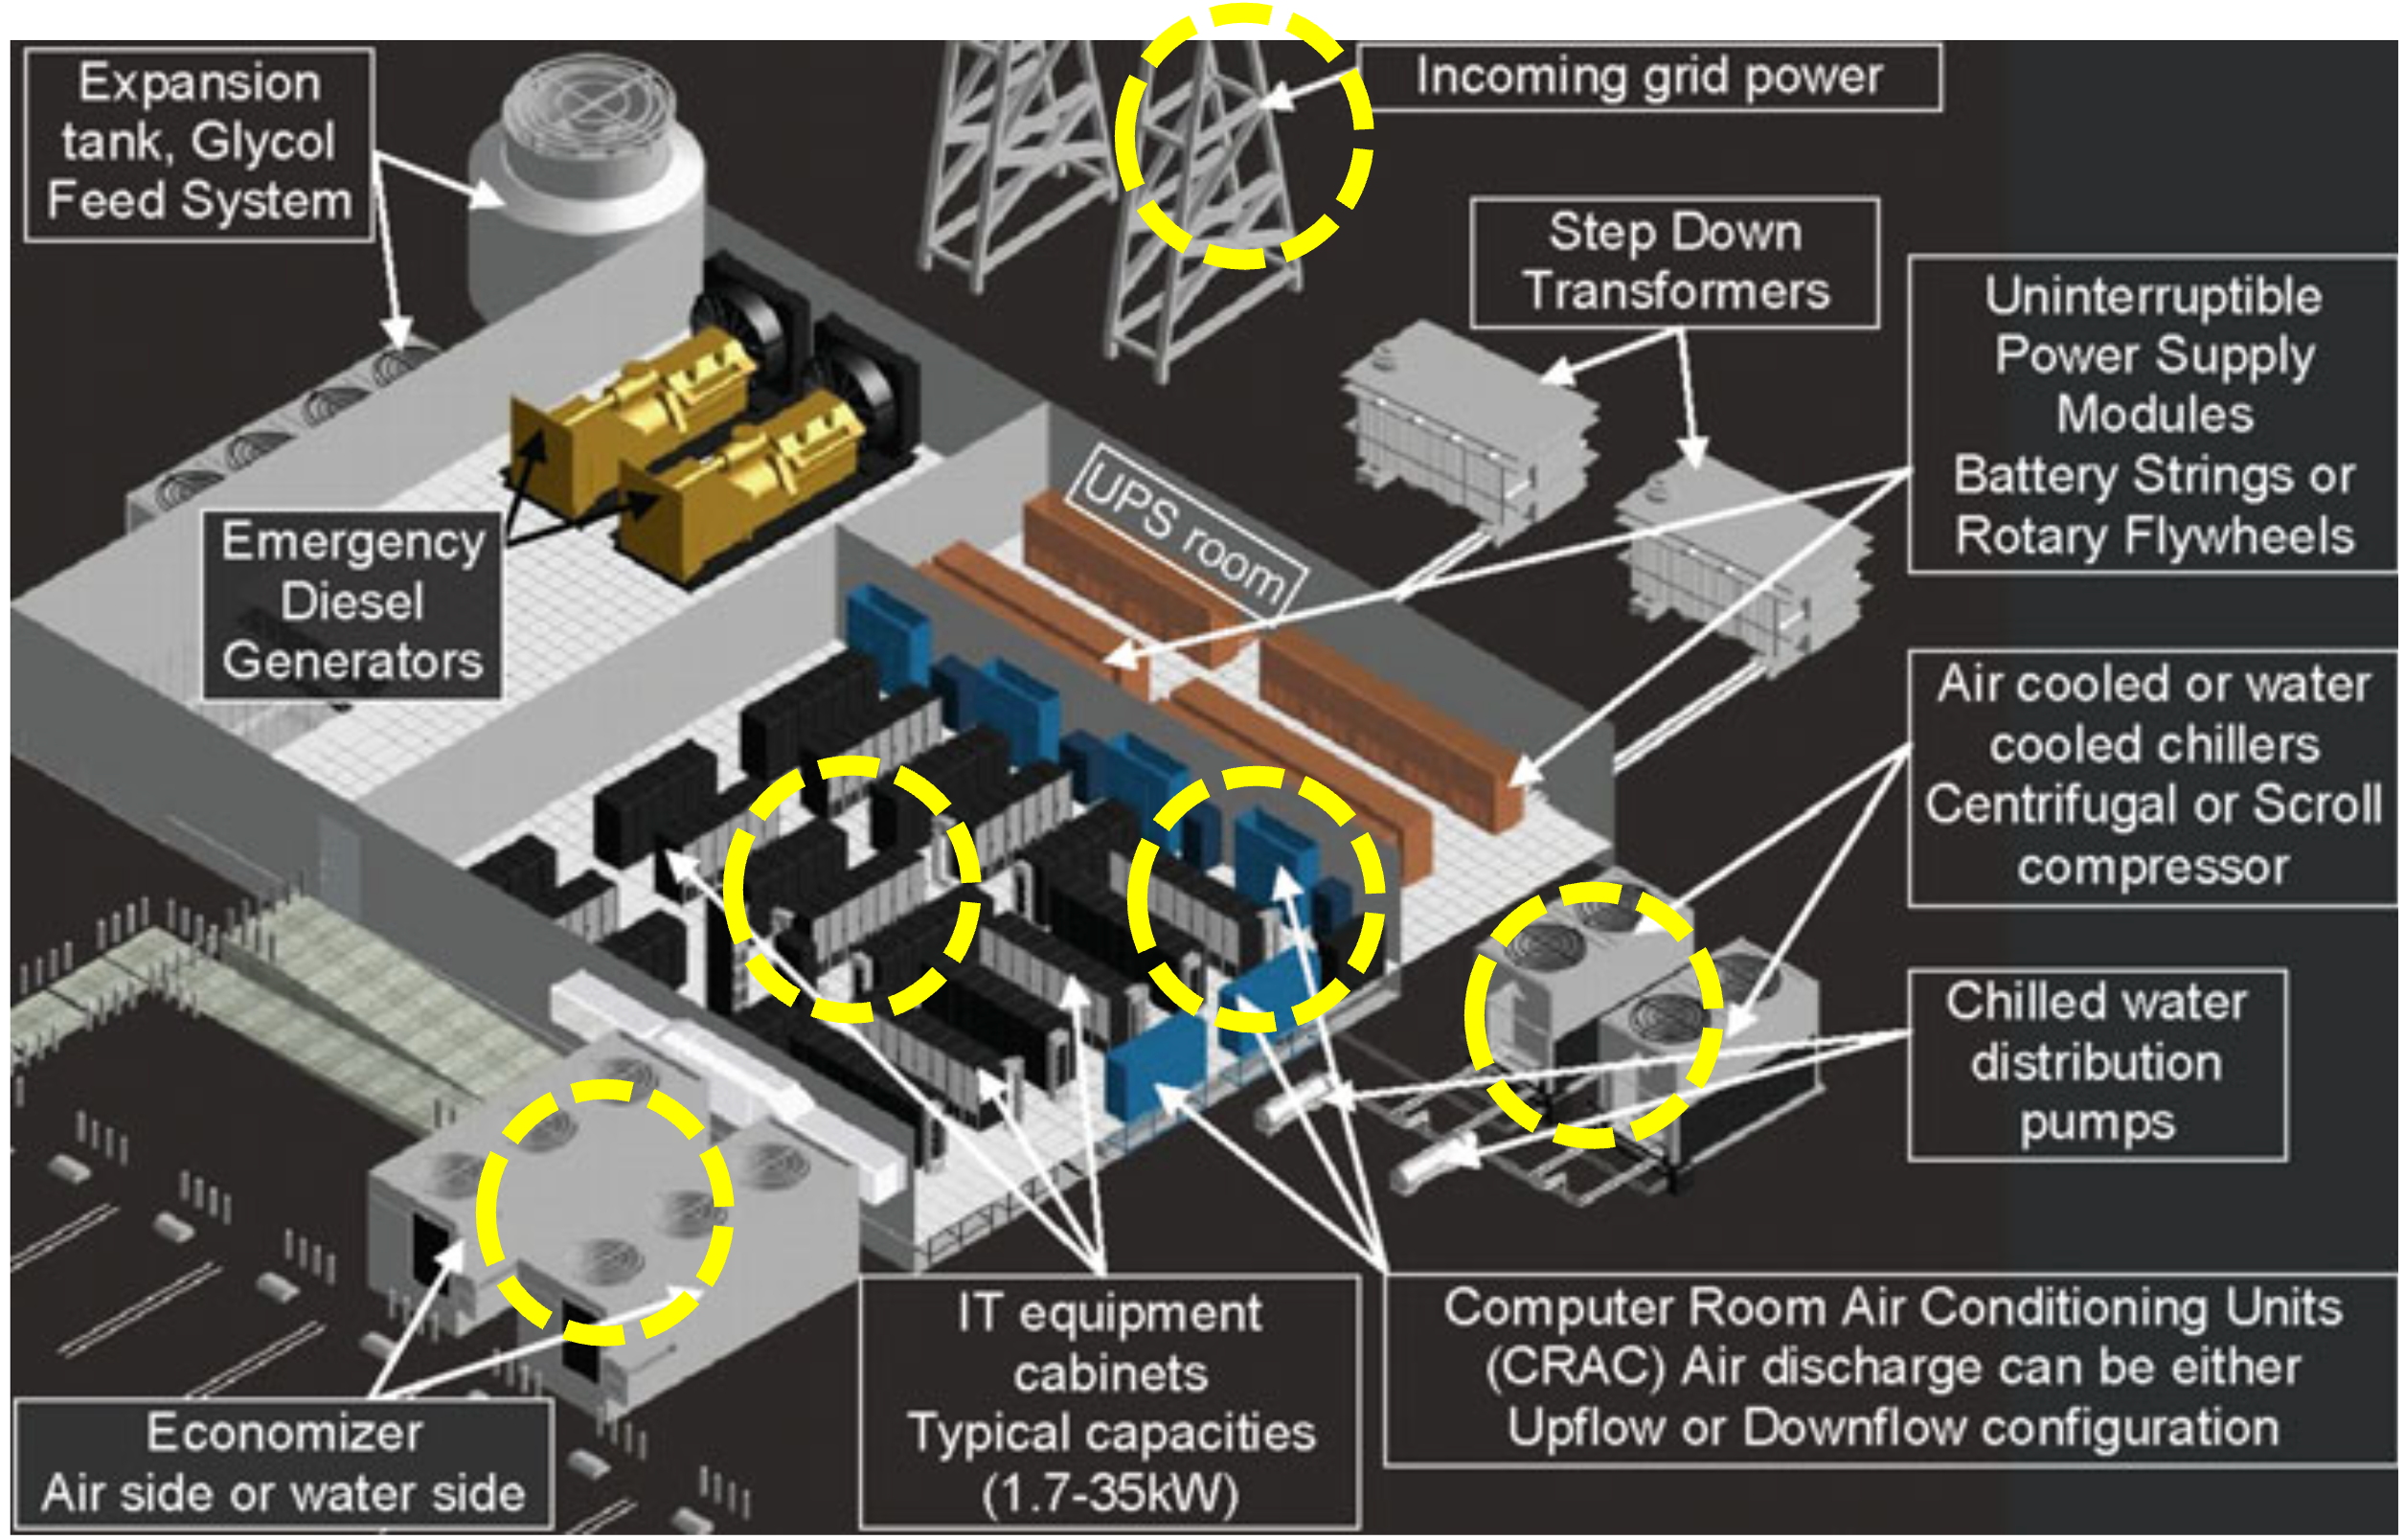
\includegraphics[width=0.65\textwidth]{../figures/joshi2021introduction-figure-01-01-L03a.png}
%			\vspace{-0.5cm}
		 \caption{(Figure 1.1 in Ref. \cite{joshi2012energy}).}
		\end{figure}
\end{frame}
}

{
\setbeamertemplate{background}{} % Hides background for this frame
\setbeamertemplate{footline}{}   % Reclaims the bottom space
\smallframetitle
\begin{frame}
	\frametitle{Simulink and Simscape}
		We can use different types of software to perform thermofluids flow network analysis. I have a few examples posted in our Github here: \href{https://github.com/mtsn-lab/me137-237a/tree/main/examples}{examples}. These run in Matlab. We can do similar things in Cadence, Modelica, etc.

\end{frame}
}

{
\setbeamertemplate{background}{} % Hides background for this frame
\setbeamertemplate{footline}{}   % Reclaims the bottom space
\smallframetitle
\begin{frame}
	\frametitle{Historical development of PUE}
2007, U.S. Environmental Protection Agency (EPA):
		\begin{itemize}
			\item ``The federal government and industry should work together to develop an objective, credible energy performance rating system for data centers, initially addressing the infrastructure portion but extending, when possible, to include a companion metric for the productivity and work output of IT equipment (ITE).''
		\end{itemize}
\end{frame}
}

{
\setbeamertemplate{background}{} % Hides background for this frame
\setbeamertemplate{footline}{}   % Reclaims the bottom space
\smallframetitle
\begin{frame}
		\frametitle{PUE}
		
		\href{https://datacenters.lbl.gov/sites/default/files/WP49-PUE\%20A\%20Comprehensive\%20Examination\%20of\%20the\%20Metric_v6.pdf}{PUE: A Comprehensive Examination of the Metric
}

\end{frame}
}

%{
%\setbeamertemplate{background}{} % Hides background for this frame
%\setbeamertemplate{footline}{}   % Reclaims the bottom space
%\smallframetitle
%\begin{frame}
%	\frametitle{ASHRAE Standards}
%		\begin{itemize}
%			\item Read Only versions of ASHRAE standards can be accessed here: \href{https://www.ashrae.org/technical-resources/standards-and-guidelines/read-only-versions-of-ashrae-standards}{link}.
%			\item See: Standard 90.4-2025 -- Energy Standard for Data Centers. 
%			\begin{itemize}
%				\item Read: mechanical load component (MLC) and electrical loss component (ELC). It regulates the efficiency of the systems that serve the data center (cooling and electrical distribution) and not the IT equipment itself.
%				\item PUE is used to report, but MLC and ELC must be used to comply. 
%			\end{itemize}
%			\item All non-data center spaces in the building must demonstrate compliance with ASHRAE Standard 90.1-2025 (see \href{https://www.energycodes.gov/comcheck}{COMcheck}).
%		\end{itemize}
%\end{frame}
%}


{
\setbeamertemplate{background}{} % Hides background for this frame
\setbeamertemplate{footline}{}   % Reclaims the bottom space
\smallframetitle
\begin{frame}
	\frametitle{ASHRAE Standards}
		\begin{itemize}
			\item Read Only versions of ASHRAE standards can be accessed here: \href{https://www.ashrae.org/technical-resources/standards-and-guidelines/read-only-versions-of-ashrae-standards}{link}.
			\item See: Standard 90.4-2025 -- Energy Standard for Data Centers. 
			\item The purpose of the standard (90.4-2025) is to establish minimum energy efficiency requirements for the design, construction, and planned operation and maintenance of data centers, and to balance those requirements with related factors affecting the environment. Factors to be evaluated include the following: 
			\begin{itemize}
				\vspace{-0.3cm}
				\item Nonrenewable energy consumption
				\item Renewable energy consumption
				\item Water consumption
				\item Greenhouse gas emissions				
			\end{itemize}
			\item The standard applies to new data centers, new additions to data centers, and modifications of data centers. 
			\item All non-data center spaces in the building must demonstrate compliance with ASHRAE Standard 90.1-2025 (see \href{https://www.energycodes.gov/comcheck}{COMcheck}).
		\end{itemize}
\end{frame}
}

{
\setbeamertemplate{background}{} % Hides background for this frame
\setbeamertemplate{footline}{}   % Reclaims the bottom space
\smallframetitle
\begin{frame}
	\frametitle{\href{https://datahub.berkeley.edu/user-redirect/git-pull?repo=https://github.com/mtsn-lab/me137-237a&subPath=examples/ashrae90-4-2025/ashrae90-4-2025.ipynb}{Annualized Mechanical Load Component and Design Electrical Loss Component (Design ELC)}}

\end{frame}
}

{
\setbeamertemplate{background}{} % Hides background for this frame
\setbeamertemplate{footline}{}   % Reclaims the bottom space
\smallframetitle
\begin{frame}
	\frametitle{Electrical distribution monitoring }
		\begin{itemize}
			\item Facility level (total building kWh, PUE):
			\begin{itemize}

				\item Smart utility meters measure the total power consumption of the entire facility. 
				\item Modern switchgears have digital meters to monitor voltage and current. 
				\item Uninterruptible power supply systems can also be used for monitoring (uptime and efficiency). 
			\end{itemize}
			
			\item Rack-level Power Monitoring (Watts per rack/outlet):
			\begin{itemize}

				\item Intelligent power distribution units. Power strips inside of the server racks. 
			\end{itemize}
			

			\item Sensors (ambient environment):
			\begin{itemize}

				\item Temperature and humidity sensors, located in the top, middle, and bottom of racks (inlet and outlet). 
				\item Airflow and differential pressure sensors.
				\item Liquid cooling flow meters.  
			\end{itemize}
			
			\item Software:
			\begin{itemize}

				\item Data center infrastructure management. Determines PUE in real-time.  
				\item Building management system, focuses on chillers, CRACs, etc. 
			\end{itemize}
		
		\end{itemize}
\end{frame}
}



{
\setbeamertemplate{background}{} % Hides background for this frame
\setbeamertemplate{footline}{}   % Reclaims the bottom space
\smallframetitle
\begin{frame}
		\frametitle{Ensemble coefficient of performance}
		



\end{frame}
}

{
\setbeamertemplate{background}{} % Hides background for this frame
\setbeamertemplate{footline}{}   % Reclaims the bottom space
\smallframetitle
\begin{frame}
\frametitle{Data center energy use}

\begin{columns}[T]

\begin{column}{0.48\textwidth}
\small
		\begin{figure}
			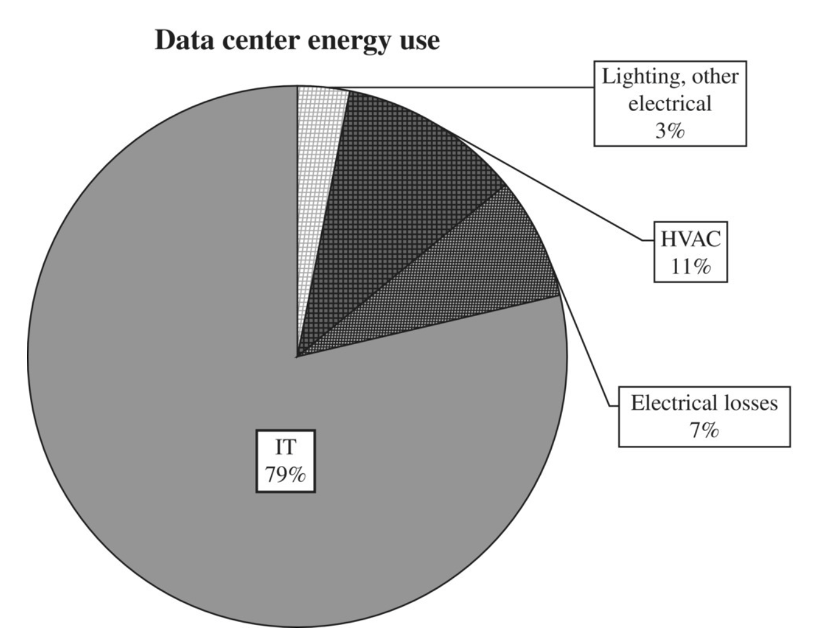
\includegraphics[width=\textwidth]{../figures/geng-data-center-energy-use.png}
			\vspace{-0.5cm}
		\caption{\label{fig:energy-use} Reproduced from Ref. \cite{geng2021data}.}
		\end{figure}


\end{column}

\begin{column}{0.48\textwidth}
	\begin{itemize}
		\item Largest power consumer in the mechanical system is the chiller. 
		\item One strategy to reduce energy use is to elevate the supply air temperature by increasing the chilled water supply temperature. 
		\item This strategy depends on the type of mechanical system, the climate, and the allowable air temperature for the IT equipment.
	\end{itemize}
\end{column}

\end{columns}
\end{frame}
}





%{
%\setbeamertemplate{background}{} % Hides background for this frame
%\setbeamertemplate{footline}{}   % Reclaims the bottom space
%\smallframetitle
%	\begin{frame}
%		\frametitle{Energy analysis of heat transfer from a cabinet}
%			\begin{itemize}
%				\item In addition to maintaining the inlet air temperatures, data centers also need to adhere to the humidity levels specified by ASHRAE guidelines.
%				\item ASHRAE: American Society of Heating, Refrigerating and Air-Conditioning Engineers
%				\item The relevant technical committee is: TC 9.9 (Mission Critical Facilities, Data Centers, Technology Spaces and Electronic Equipment): The flagship committee for data centers. TC 9.9 sets global industry standards for thermal guidelines. 
%				\item Standard 90.1-2025 -- Energy Standard for Data Centers: \href{https://ashrae.iwrapper.com/ASHRAE_PREVIEW_ONLY_STANDARDS/STD_90.4_2025}{Link}. You need to register in order to read. You can also become a student member of ASHRAE. There is a Golden Gate chapter. 
%		\end{itemize}
%	\end{frame}
%}

%{
%\setbeamertemplate{background}{} % Hides background for this frame
%\setbeamertemplate{footline}{}   % Reclaims the bottom space
%\smallframetitle
%\begin{frame}{The ideal vapor-compression refrigeration cycle}
%  \begin{columns}
%    \begin{column}{0.48\textwidth}
%		\begin{figure}
%			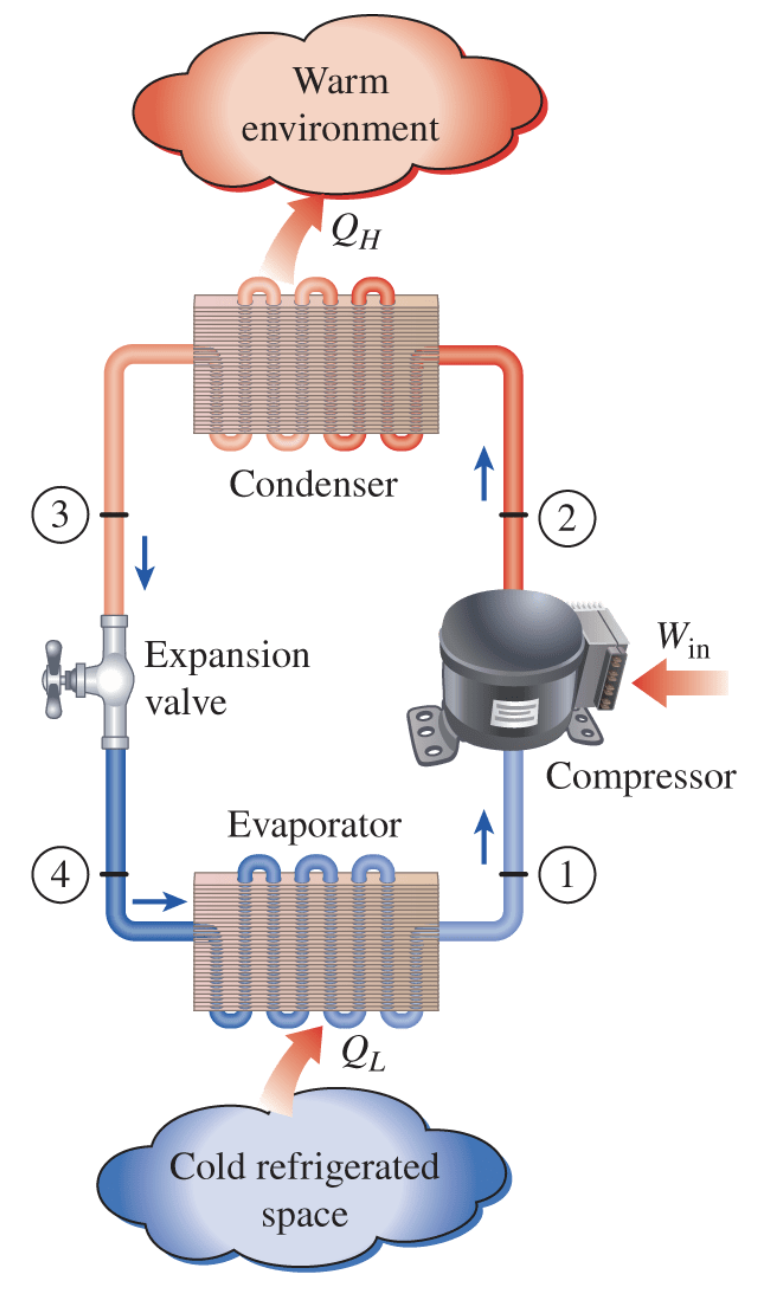
\includegraphics[width=0.5\textwidth]{../figures/cengel2019thermodynamics-figure-11-3.png}
%%			\vspace{-0.5cm}
%		 \caption{\label{fig:refrigeration-system}Reproduced from Figure 11.3 in Ref. \cite{cengel2019thermodynamics}.}
%		\end{figure}
%    \end{column}
%
%    \begin{column}{0.48\textwidth}
%		\begin{figure}
%			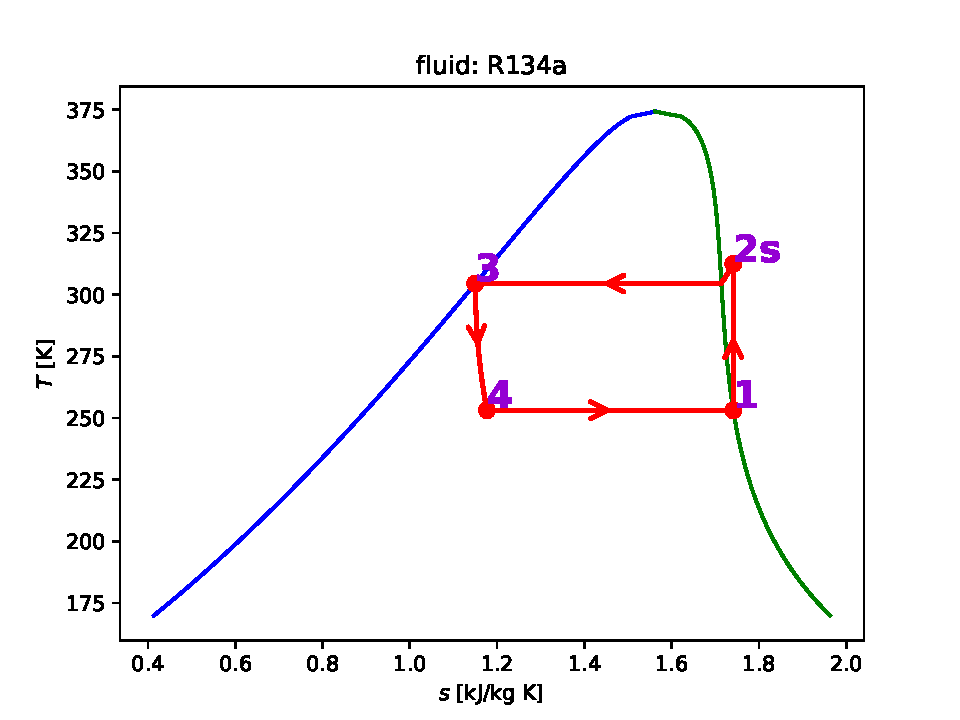
\includegraphics[width=1\textwidth]{../figures/refrigerationCycleR134a_Ts.pdf}
%%			\vspace{-0.5cm}
%		 \caption{\label{fig:refrigeration-system}Generated from \href{https://datahub.berkeley.edu/user-redirect/git-pull?repo=https://github.com/mtsn-lab/me40&subPath=scripts/refrigerationCycleR134a.ipynb}{here}.}
%		\end{figure}
%    \end{column}
%  \end{columns}
%\end{frame}
%}



{
\setbeamertemplate{background}{} % Hides background for this frame
\setbeamertemplate{footline}{}   % Reclaims the bottom space
\setbeamertemplate{bibliography item}[text] % Replaces default icons with numbers
\smallframetitle
	\begin{frame}[allowframebreaks]{References}
		\bibliographystyle{plain}
		\bibliography{../../bibliography}
	\end{frame}
}

%{
%\setbeamertemplate{background}{} % Hides background for this frame
%\setbeamertemplate{footline}{}   % Reclaims the bottom space
%\smallframetitle
%\begin{frame}
%\frametitle{Teaching team}
%
%\begin{columns}[T]
%
%\begin{column}{0.48\textwidth}
%\small
%Ben Brown
%
%		\begin{figure}
%			
\includegraphics[width=0.5\textwidth]{figures/ben-brown.pdf}
%			\vspace{-0.5cm}
%%		\caption{\label{fig:ben-brown}\href{https://eta-publications.lbl.gov/sites/default/files/2024-12/lbnl-2024-united-states-data-center-energy-usage-report.pdf}{eta-publications.lbl.gov}}
%		\end{figure}
%
%
%\end{column}
%
%\begin{column}{0.48\textwidth}
%Amelia Stacey
%
%		\begin{figure}
%			
\includegraphics[width=0.5\textwidth]{figures/oski.jpeg}
%			\vspace{-0.5cm}
%%		\caption{\label{fig:ben-brown}\href{https://eta-publications.lbl.gov/sites/default/files/2024-12/lbnl-2024-united-states-data-center-energy-usage-report.pdf}{eta-publications.lbl.gov}}
%		\end{figure}
%\end{column}
%
%\end{columns}
%\end{frame}
%}




\end{document}
